\chapter{Introduction}

\epigraph{``And now you're asking, I don't know where to begin''}{{\sl Mike Vennart, Silent/Transparent}}
%
%“We demand rigidly defined areas of doubt and uncertainty!” 
%― Douglas Adams, The Hitchhiker's Guide to the Galaxy

The release of gravitational potential energy as mass falls towards
a compact object is the most efficient energetic process in the universe,
capable of liberating more rest mass energy than nuclear fusion.
This {\em accretion} process is thought to power the huge radiative engines at the 
centres of every galaxy -- accreting supermassive black holes known as active galactic nuclei (AGN). 
In addition to AGN, accretion discs are seen in X-ray binaries (XRBs), young-stellar objects (YSOs) and
accreting white dwarfs (AWDs). Accretion therefore appears to be a universal process; broadly speaking, the physics is the same whether it is taking place in a $\sim1~M_\odot$ Neutron Star or White Dwarf 
system, or a $\sim10^{10}~M_\odot$ black hole -- a {\em quasar}.

Outflows are ubiquitous in accreting systems. We see collimated radio jets in AGN (REF) and
XRBs (REF), and there is even evidence of extended radio emission in AWDs (REF). These radio jets
tend to appear in specific accretion states (REF), implying an intrinsic connection to the 
accretion process. Even more intriguing, in XRBs less collimated, mass-loaded outflows
or {\em winds} are observed in the opposite accretion state, possibly emanating from the accretion disc.
Evidence for disc winds is widespread across the mass range, but perhaps the most spectacular indication
is the blue-shifted, broad absorption lines (BALs) in the rest-frame ultraviolet (UV)
seen in high-state AWDs (REFs) and so-called broad absorption line quasars seen in $20-40\%$
of quasars (BALQSOs; REFs). 

The astrophysical significance of disc winds extends, quite literally, 
far beyond the accretion environment. They offer a potential mechanism by which the central
accretion engine can interact with the host galaxy and interstellar medium (REFs). 
This is often referred to as AGN feedback (REF), and is required in models of 
galaxy evolution

This thesis is structured as follows. In the remainder of this chapter, 
I shall describe the different classes of accretion systems. In chapter 2, 
I will give the background accretion theory and detail the successes and failures
of accretion disc models when compared to observations, before 
discussing the outflows associated with accretion discs in chapter 3. Chapter 4
outlines the Monte Carlo radiative transfer (MCRT) and photoionization
methods I have used in order to investigate the impact of disc 
winds on the spectra of accreting systems. The science chapters
contain three separate submitted papers, in which we investigated the impact
of disc winds on the spectra of CVs (Chapter 5), and tested the disc winds
quasar unification model (Chapters 6 and 7).
In chapter 8, I summarise my findings and their astrophysical significance, 
and discuss potential avenues for future work.


\section{Types of Accreting Systems}

\subsection{Cataclysmic Variables}
Cataclysmic variables (CVs) are systems in which a white dwarf
accretes matter from a donor star via Roche-lobe overflow. In
non-magnetic systems this accretion is mediated by a Keplerian disc
around the white dwarf (WD). Nova-like variables (NLs) are a subclass
of CVs in which the  disc is always in a relatively
high-accretion-rate state ($\dot{M} \sim 10^{-8}$~M$_{\odot}$~yr$^{-1}$).  
This makes NLs an excellent laboratory for studying the properties of 
steady-state accretion discs. 

\subsection{X-ray Binaries}
X-ray binaries are similar to CVs in structure, except that the compact object
is either a neutron star (NS) or black hole (BH). The accretion disc 
emits in the soft X-rays, and an additional hard X-ray power law is also 
seen in the spectrum (REFs). This hard component is normally attributed
to Compton up-scattering of seed disc photons by some kind of `corona'
of hot electrons close to the BH (REFs). 

Although I do not discuss XRBs directly in this thesis, it is instructive
to discuss some of their observational appearance as it is instructive 
for understanding the theory of disc winds, as well as their wider significance. 
The discovery that XRBs follow similar tracks on a hardness-intensity diagram (REFs)
is particularly interesting in this regard, especially since Ponti et al. (2012)
showed that broad Fe absorption lines are only seen in the soft-state 
high-inclination systems, implying that equatorial outflows are intrinsic to 
the accretion process (see figure~\ref{fig:ponti_cartoon}). Although the driving mechanism
is almost certainly different to CVs (REFs), the similarity in general structure 
to models for CVs and quasars is striking.

\begin{figure}
\centering
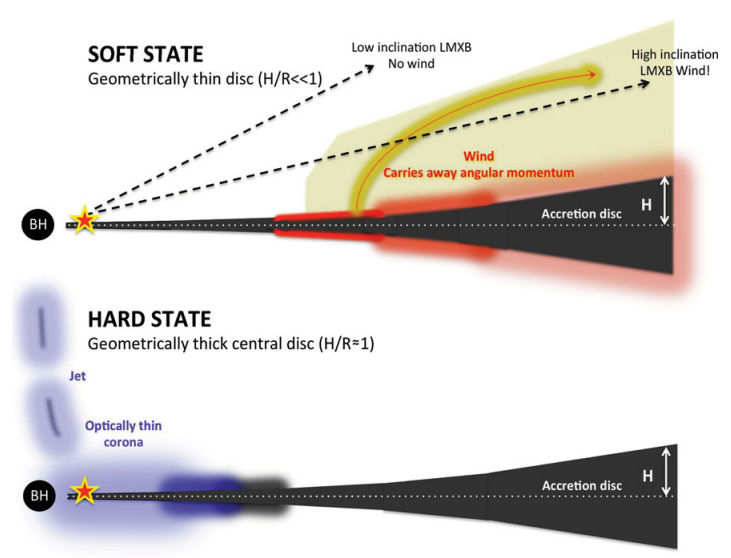
\includegraphics[width=0.7\textwidth]{figures/ponti_wind_cartoon.png}
\caption
[Hardness intensity diagram for a WD, NS and BH system]
{
{\sl Credit: Ponti et al. 2012}
Hardness intensity diagram for a WD, NS and BH system
} 
\label{fig:ponti_cartoon}
\end{figure}

\subsection{Quasars and Active Galactic Nuclei}



